% Bản thảo paper. Số liệu ở mục Results lấy từ results/tables/*.csv; chỗ \todo{} là chưa có số.
\documentclass[conference]{IEEEtran}
\usepackage{graphicx,booktabs,amsmath,url,xcolor}
\usepackage[hidelinks]{hyperref}
\newcommand{\todo}[1]{\textcolor{red}{[TODO: #1]}}
\graphicspath{{../results/figures/}}

\begin{document}
% Tiêu đề tạm (2026-10-28): hướng benchmark, trung tính; có thể chỉnh sau khi viết xong Results
\title{Benchmarking Statistical, Machine Learning and Deep Learning Models for Daily Retail Revenue Forecasting Across Multiple Regions}
\author{\IEEEauthorblockN{\todo{authors}}\IEEEauthorblockA{\todo{affiliation}}}
\maketitle

% ---------------------------------------------------------------- 4.1
\begin{abstract}
Accurate daily revenue forecasts support inventory, staffing and financial planning in retail, yet published comparisons of forecasting models often differ in data, horizons and inputs, which makes their conclusions hard to transfer.
This study benchmarks ten widely used models---ARIMA, SARIMA, SARIMAX, Prophet, Random Forest, Gradient Boosting, XGBoost, LightGBM, RNN and LSTM---together with seasonal-naive baselines and three forecast-combination schemes, on daily revenue and cost of goods sold (COGS) of an e-commerce retailer, aggregated to a national total and three regions (3{,}833 days, 2012--2022).
All models receive the same calendar, promotion and regime covariates, and each is also run in a ``pure'' autoregressive form to isolate the value of this information.
Models are tuned and compared with four-fold expanding-window time-series cross-validation and evaluated once on an 18-month hold-out test set using RMSE, MAE and MAPE, with Diebold--Mariano and Friedman--Nemenyi tests.
\todo{main results: best model, gain over baseline, ablation gain, ensemble gain}.
\todo{contribution sentence}.
\end{abstract}

\begin{IEEEkeywords}
retail sales forecasting, time series cross-validation, gradient boosting, LSTM, forecast combination, calendar effects
\end{IEEEkeywords}

% ---------------------------------------------------------------- 4.2
\section{Introduction}
Forecasting total sales is a routine but consequential task in retail: daily forecasts drive replenishment, workforce scheduling and cash-flow planning, and their errors propagate into stock-outs, waste and missed revenue~\cite{fildes2022retail}.
Large forecasting competitions on retail data, such as M5 on Walmart sales~\cite{makridakis2022m5}, have shown the strength of tree-based machine learning, while many applied studies report conflicting winners among ARIMA, Prophet, LSTM and gradient boosting~\cite{hasan2022comparative,ensafi2022seasonal,hobor2026comparative}.

Daily retail revenue is hard to forecast over long horizons for several reasons that appear together in our data: strong annual seasonality, intra-month patterns, promotion campaigns that recur on fixed calendar dates (some only in odd years), and a structural break that lowers the level of the series by about 40\%.
Data from multiple regions add a further question: whether to forecast the total directly or to aggregate regional forecasts~\cite{hyndman2011hierarchical}.

\todo{limitations of existing comparisons: different inputs per model; short horizons; recursive strategies; single split; no significance testing}.

The objectives of this study are to
(i) compare nine forecasting models from three families under one protocol for horizons up to 18 months;
(ii) measure how much of the accuracy comes from known-in-advance calendar information rather than from model class;
(iii) evaluate whether forecast combination improves on the best single model; and
(iv) compare direct and bottom-up forecasting of the total from three regional series.
\todo{contributions list after results}.

% ---------------------------------------------------------------- 4.3
\section{Related Work}
\subsection{Statistical models}
ARIMA-type models remain the reference for univariate forecasting; for long seasonal periods such as daily data with annual seasonality, Fourier terms with ARMA errors (dynamic harmonic regression) are the practical form of seasonal ARIMA~\cite{hyndman2021fpp3}.
Prophet decomposes a series into trend, seasonality and holiday effects~\cite{taylor2018prophet}.
\subsection{Machine learning}
Random forests~\cite{breiman2001rf} and gradient boosting~\cite{friedman2001gbm}, with its scalable implementations XGBoost~\cite{chen2016xgboost} and LightGBM~\cite{ke2017lightgbm}, are now standard for retail demand forecasting~\cite{januschowski2022trees,makridakis2022m5,spiliotis2020sku}.
Calendar-related special days are a key input for daily retail demand~\cite{huber2020calendric}.
\subsection{Deep learning}
Recurrent networks~\cite{elman1990rnn} and LSTM~\cite{hochreiter1997lstm} have been applied to sales forecasting~\cite{bandara2019lstm}; a review of RNNs for forecasting is given in~\cite{hewamalage2021rnn}.
\subsection{Forecast combination and evaluation}
Combining forecasts dates back to~\cite{bates1969combination}; see~\cite{clemen1989combining,wang2023combinations} for reviews and~\cite{wolpert1992stacked} for stacking.
For time series, cross-validation must respect temporal order~\cite{tashman2000outofsample,bergmeir2012cv,bergmeir2018cv}; forecast accuracy comparisons can be tested with the Diebold--Mariano test~\cite{diebold1995dm,harvey1997hln} and, across many problems, with Friedman--Nemenyi ranks~\cite{demsar2006statistical}.
\subsection{Research gap}
\todo{write after reading full texts in literature\_matrix.csv: few studies give all model families the same covariates, use long horizons with direct (non-recursive) strategies, and test significance}.

% ---------------------------------------------------------------- 4.4
% Mọi chi tiết ở mục này lấy từ protocol.md và src/rsf/ (đúng với lần chạy CV/test trên Colab).
\section{Methodology}
\subsection{Data}
The data are the order-level transactions of an online retailer released for Datathon 2026 \todo{describe retailer, product range, currency and data licence}.
For this study, the series were extracted from a data warehouse built on the competition data (release \texttt{ccde5a5e}); we verified that all four series and the promotion calendar are identical, to within $1.3\times10^{-8}$, to those rebuilt directly from the raw files.
Daily revenue is $\sum$ quantity $\times$ unit price (before discounts, over orders of all statuses) and daily COGS is $\sum$ quantity $\times$ unit cost.
Each order is assigned to one of three regions (East, Central, West) through its postal code; the regions account for 46.5\%, 30.1\% and 23.4\% of total revenue, and the three regional series sum exactly to the national total.
This gives four series (Total and three regions) and two targets (revenue and COGS), each covering 3{,}833 consecutive days from 4 July 2012 to 31 December 2022 with no missing or non-positive values (Fig.~\ref{fig:series}).

The series combine several features that make long-horizon forecasting difficult.
They have strong annual seasonality and intra-month patterns.
Six promotion campaigns recur on nearly fixed calendar dates: four every year and two (\emph{Urban Blowout} in August and \emph{Rural Special} around February) only in odd years.
There is also a level shift at the end of 2018: mean daily revenue fell from 5.07 million in 2018 to 3.11 million in 2019 ($-39\%$) and stayed at the lower level.

\begin{figure}[t]\centering
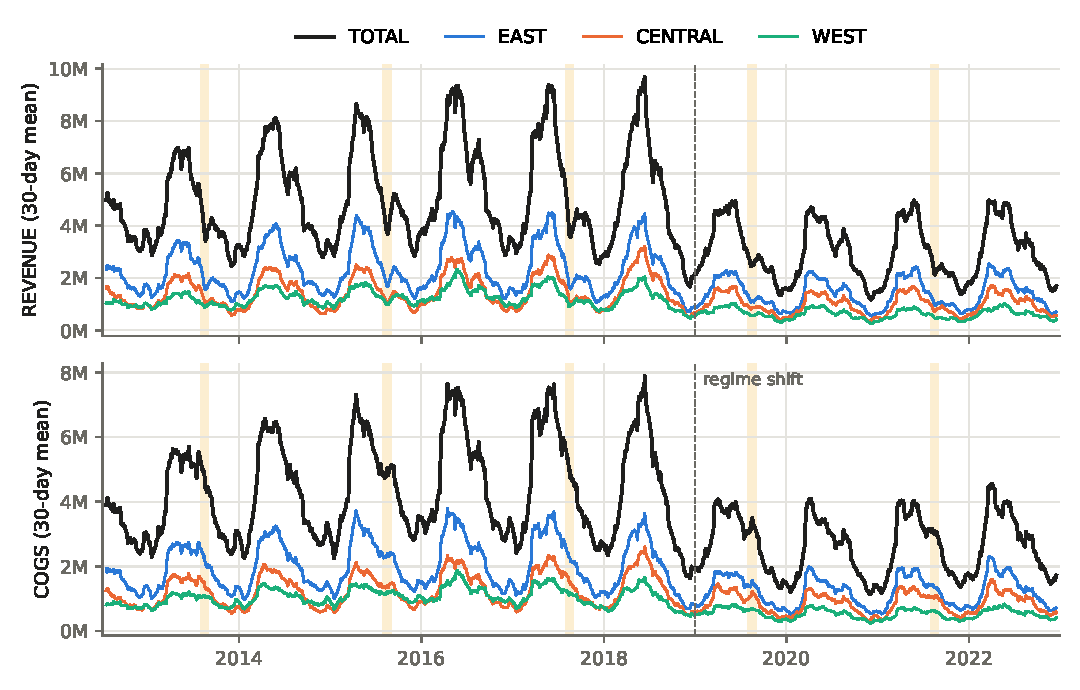
\includegraphics[width=\columnwidth]{F01_series.pdf}
\caption{Daily revenue and COGS (30-day mean) for the total and three regions. Shaded: odd-year August promotion; dashed: regime shift (2019).}\label{fig:series}
\end{figure}

\subsection{Forecasting task}
Let $T$ be a forecast origin, the last day whose value is observed.
Each model is fitted on $y_1,\dots,y_T$ and then produces $\hat y_{T+1},\dots,\hat y_{T+H}$ in a single pass, without re-estimation and without access to actual values inside the horizon.
The horizon is $H=365$ days in cross-validation and $H=549$ days on the test set.
Every model is fitted separately to each of the eight series--target pairs.
All models except the seasonal-naive baselines are fitted to $\log y_t$, and forecasts are transformed back with $\exp(\cdot)$ before evaluation.

\subsection{Covariates}
All covariates are known in advance at the forecast origin (Table~\ref{tab:covariates}).
Day-of-week effects were excluded because they explain almost no variance in the daily series ($R^2=0.008$ in a prior analysis of the same data).
Two variants of the covariate set are used.
The \emph{linear} set is used by SARIMAX and by Prophet, which uses its own yearly seasonality instead of the Fourier terms.
The \emph{tree} set adds ordinal and campaign-progress variables and is used by the tree ensembles and by RNN/LSTM.

\begin{table}[t]\centering
\caption{Covariate groups. L: linear set; T: tree set.}\label{tab:covariates}
\footnotesize
\begin{tabular}{@{}llc@{}}
\toprule
Group & Variables & Set \\
\midrule
Annual seasonality & Fourier terms of day of year, $K=5$ (10 terms) & L, T \\
 & month, day of year & T \\
Intra-month (\emph{dom}) & days to end of month; first/last 1--3 days of month & L, T \\
 & day of month & T \\
Promotions (\emph{promo}) & six campaign indicators & L, T \\
 & days since campaign start; odd-year indicator & T \\
Regime & post-2019 indicator & L, T \\
\bottomrule
\end{tabular}
\end{table}

Two rules prevent information from after the origin leaking into the covariates.
First, campaign windows for future dates are extrapolated from the calendar dates of campaigns that started on or before the origin; a campaign observed at least twice and only in odd years is switched on only in odd years.
Second, the post-2019 indicator is included only when at least 180 days after 1 January 2019 have been observed, i.e.\ for origins from mid-2019 onwards (folds F3, F4 and the test set).
The break date itself comes from exploratory analysis of the full series in a previous project; we return to this in the discussion of limitations.

\subsection{Models}
Table~\ref{tab:models} lists the ten main models, grouped into three families, and the two baselines.
\begin{itemize}
\item \emph{Baselines.} Seasonal naive forecasts copy the value on the same calendar day one year earlier (SNaive-1Y) or two years earlier (SNaive-2Y). SNaive-2Y keeps the odd/even-year parity of the odd-year campaigns.
\item \emph{Statistical models.} ARIMA uses no covariates; its order is chosen by AIC over $p,q\in\{0,1,2\}$, $d\in\{0,1\}$, with a constant when $d=0$. A seasonal ARIMA with period 365 is impractical, so SARIMA is implemented as dynamic harmonic regression, i.e.\ Fourier terms with ARMA errors~\cite{hyndman2021fpp3}. SARIMAX extends it with the full linear covariate set. Prophet~\cite{taylor2018prophet} uses its yearly seasonality plus the linear covariates (except Fourier terms) as additive regressors, with weekly and daily seasonality disabled.
\item \emph{Machine learning.} Random Forest~\cite{breiman2001rf}, histogram-based Gradient Boosting~\cite{friedman2001gbm} (scikit-learn), XGBoost~\cite{chen2016xgboost} and LightGBM~\cite{ke2017lightgbm} regress $\log y_t$ directly on the covariates of day $t$. They use no lagged values of the target, so a single fitted model produces forecasts for any horizon and errors do not accumulate along the horizon.
\item \emph{Deep learning.} The Elman RNN~\cite{elman1990rnn} and LSTM~\cite{hochreiter1997lstm} take a window of the standardized tree covariates of the $L$ days ending at $t$. One recurrent layer and a linear output layer map this window to the standardized $\log y_t$, again without lagged target values. Networks are trained with Adam (learning rate $10^{-3}$, batch size 64, mean squared error). The number of epochs is chosen by early stopping on the last 10\% of the training period (patience 25, at most 300 epochs), and the network is then refitted on the full training period for that number of epochs. Each network is trained with five seeds; the reported forecast is the mean of the five seed forecasts, and the spread across seeds is reported separately.
\end{itemize}

\begin{table*}[t]\centering
\caption{Models, inputs, forecasting strategy and hyperparameter grids. Selected values (bold) are the configurations with the lowest mean MAE over the four CV folds on Total revenue.}\label{tab:models}
\footnotesize
\begin{tabular}{@{}lllll@{}}
\toprule
Model & Family & Inputs & Strategy & Grid (selected value in bold) \\
\midrule
SNaive-1Y / SNaive-2Y & baseline & target & copy same day 1 / 2 years earlier & -- \\
ARIMA & statistical & target & state space, multi-step & order by AIC on each training set \\
SARIMA & statistical & Fourier & regression with ARMA errors & ARMA $(p,q)\in\{(1,1),\mathbf{(2,1)},(1,2),(2,2)\}$ \\
SARIMAX & statistical & linear set & regression with ARMA errors & ARMA $(p,q)\in\{(1,1),(2,1),(1,2),\mathbf{(2,2)}\}$ \\
Prophet & statistical & linear set$^{a}$ & additive decomposition & growth $\in\{\mathbf{flat},\text{linear}\}$, changepoint scale $\in\{\mathbf{0.01},0.05,0.5\}$ \\
Random Forest & ML & tree set & direct regression & 500 trees; min leaf $\in\{1,\mathbf{3},10\}$, max features $\in\{0.33,0.5,\mathbf{1.0}\}$ \\
Gradient Boosting & ML & tree set & direct regression & 500 iterations; learning rate $\in\{\mathbf{0.03},0.1\}$, max leaf nodes $\in\{\mathbf{7},15,31\}$ \\
XGBoost & ML & tree set & direct regression & 800 trees; learning rate $\in\{\mathbf{0.03},0.1\}$, max depth $\in\{\mathbf{3},4,6\}$ \\
LightGBM & ML & tree set & direct regression & 800 trees; learning rate $\in\{\mathbf{0.03},0.1\}$, leaves $\in\{\mathbf{7},15,31\}$, min child $\in\{10,\mathbf{30}\}$ \\
RNN & DL & tree set, window $L$ & sequence-to-one & hidden $\in\{16,\mathbf{32},64\}$, $L\in\{14,28,\mathbf{56}\}$ \\
LSTM & DL & tree set, window $L$ & sequence-to-one & hidden $\in\{16,32,\mathbf{64}\}$, $L\in\{14,28,\mathbf{56}\}$ \\
\bottomrule
\multicolumn{5}{@{}l}{\scriptsize $^{a}$ Without Fourier terms; Prophet's own yearly seasonality is used instead.}
\end{tabular}
\end{table*}

To show where the accuracy of the main models comes from, we also run two kinds of ablation.
\begin{itemize}
\item \emph{Pure variants} use no calendar information and forecast recursively, with default (untuned) hyperparameters:
\begin{itemize}
\item SARIMA with weekly seasonality, $(1,1,1)\times(1,0,1)_7$;
\item Prophet with default settings;
\item each tree model on target lags $\{1,2,3,7,14,28,30,60,90,180,365\}$ and rolling means over $\{7,28,90\}$ days;
\item RNN and LSTM on the last 56 values of the target (three seeds).
\end{itemize}
\item \emph{Feature-group ablations} remove one covariate group (regime, promo or dom; Table~\ref{tab:covariates}) from SARIMAX and from LightGBM and keep their tuned hyperparameters.
\end{itemize}

\subsection{Hyperparameter tuning}
Each tuned model has a grid of at most 12 configurations, fixed before tuning (Table~\ref{tab:models}).
Every configuration is evaluated on the Total revenue series over the four cross-validation folds with one seed.
The configuration with the lowest mean MAE is then used for all series and targets.
The test set is never used for tuning or for any other choice.

\subsection{Evaluation protocol}
We use rolling-origin evaluation with an expanding training window~\cite{tashman2000outofsample,bergmeir2018cv} (Fig.~\ref{fig:splits}).
\begin{itemize}
\item \emph{Cross-validation} has four folds, with origins on 30 June of 2017, 2018, 2019 and 2020. Each fold scores the 365 days after its origin, and training always starts on 4 July 2012. Fold F2 contains the 2018 level shift.
\item \emph{Test.} The test origin is 30 June 2021, and the test set (1 July 2021 to 31 December 2022, 549 days) was forecast and scored once, after the proposed method and the combination rules had been fixed.
\end{itemize}

\begin{figure}[t]\centering
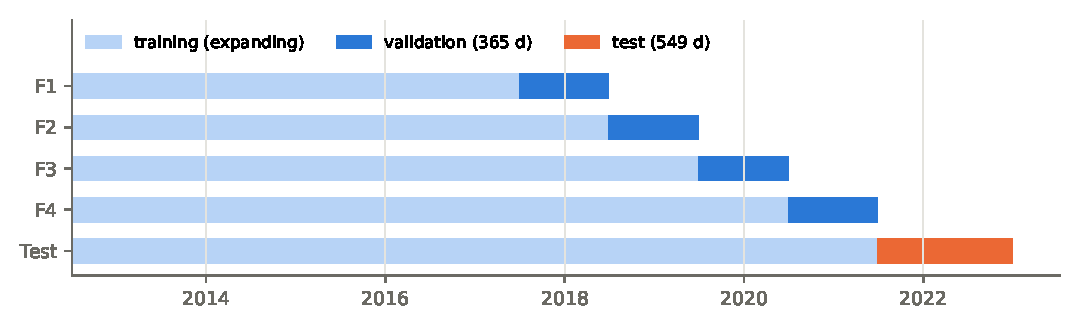
\includegraphics[width=\columnwidth]{F03_splits.pdf}
\caption{Expanding-window cross-validation folds and hold-out test set.}\label{fig:splits}
\end{figure}

Accuracy is measured on the original scale over the $n$ scored days:
\begin{gather*}
\mathrm{MAE}=\tfrac1n\textstyle\sum_t|y_t-\hat y_t|,\qquad
\mathrm{RMSE}=\sqrt{\tfrac1n\textstyle\sum_t(y_t-\hat y_t)^2},\\
\mathrm{MAPE}=\tfrac{100}{n}\textstyle\sum_t|y_t-\hat y_t|/y_t .
\end{gather*}
MAPE is well defined because all values are positive.
Errors are also broken down by lead time (1--30, 31--90, 91--365 and 366--549 days) and for the odd-year August campaign.

The folds share training data and are therefore not independent.
For this reason we report the mean and standard deviation across folds, and do not use paired $t$-tests across folds.
Models are compared with two statistical tests:
\begin{itemize}
\item On cross-validation, the Friedman test with the Nemenyi post-hoc test~\cite{demsar2006statistical} ($\alpha=0.05$) ranks the ten main models and two baselines over the 16 revenue problems (four series $\times$ four folds).
\item On the test set, each model is compared with the most accurate model of the same series and target using the Diebold--Mariano test~\cite{diebold1995dm} on absolute errors, with the small-sample correction of Harvey et al.~\cite{harvey1997hln}. \todo{state the long-run variance estimator once the autocorrelation-robust version is adopted}
\end{itemize}

\subsection{Forecast combination}
Majority voting applies to classification; its regression analogue is forecast averaging.
We combine the ten main models in three ways:
\begin{itemize}
\item the equal-weight average of the three models with the lowest MAE;
\item inverse-MAE weights over the same three models;
\item stacking~\cite{wolpert1992stacked} by non-negative least squares on out-of-fold forecasts, with weights normalised to sum to one.
\end{itemize}
To avoid look-ahead, the weights for fold F$k$ are learned only from the forecasts of the folds before it. F1 has no earlier fold and therefore uses the equal-weight average of all ten models. Weights for the test set are learned from all four folds.

Comparing a combination with the single model that turns out best in hindsight would favour the single model.
Instead, the reference is a single model chosen by the same online rule, namely the model with the lowest MAE on the earlier folds.
Combinations are therefore compared on folds F2--F4.

\subsection{Multi-region and COGS forecasts}
For each model, the \emph{bottom-up} forecast of the total is the sum of its three regional forecasts, and it is compared with the model's direct forecast of the total~\cite{hyndman2011hierarchical}.
COGS is forecast directly, and also indirectly as forecast revenue multiplied by the COGS-to-revenue ratio for each month and for the presence of the August campaign, learned on the training period.

\subsection{Choice of the proposed method}
The selection rule was fixed in the protocol before cross-validation: the proposed method is the model with the lowest mean CV MAE on revenue, averaged over the four series.
This rule selected the RNN (mean of five seeds), and the choice was recorded before the test set was opened.
The test set is nonetheless reported for every model, so that the selected method can be compared with all alternatives on unseen data.

% ---------------------------------------------------------------- 4.5
\section{Experiments and Results}
\subsection{Setup}
\todo{hardware, library versions from results/env\_*.json, runtime table T8}.
\subsection{Cross-validation results}
\todo{Table T1, Fig. F04, F05}.
\subsection{Value of calendar information}
\todo{Table T2, Fig. F06}.
\subsection{Forecast combination}
\todo{T1 ensemble rows}.
\subsection{Multi-region: direct vs. bottom-up}
\todo{T4, Fig. F09}.
\subsection{Test-set results}
\todo{T1 test columns, T7 DM tests, Fig. F10, F11}.
\subsection{Discussion}
\todo{error by lead time (F08), odd-year August (T6), COGS direct vs ratio (T5), limitations: single retailer, retrospective benchmark}.

\section{Conclusion}
\todo{}

\bibliographystyle{IEEEtran}
\bibliography{refs}
\end{document}
